\documentclass{article}
\usepackage{graphicx}
\graphicspath{ {src/image/} }

\begin{document}

\title{A Sample \LaTeX{} Document}
\author{Author's Name}

\maketitle

\begin{abstract}
The abstract text goes here.
\end{abstract}

\section{Introduction}
Here is some introductory copy.

This is a reference\cite{einstein}.


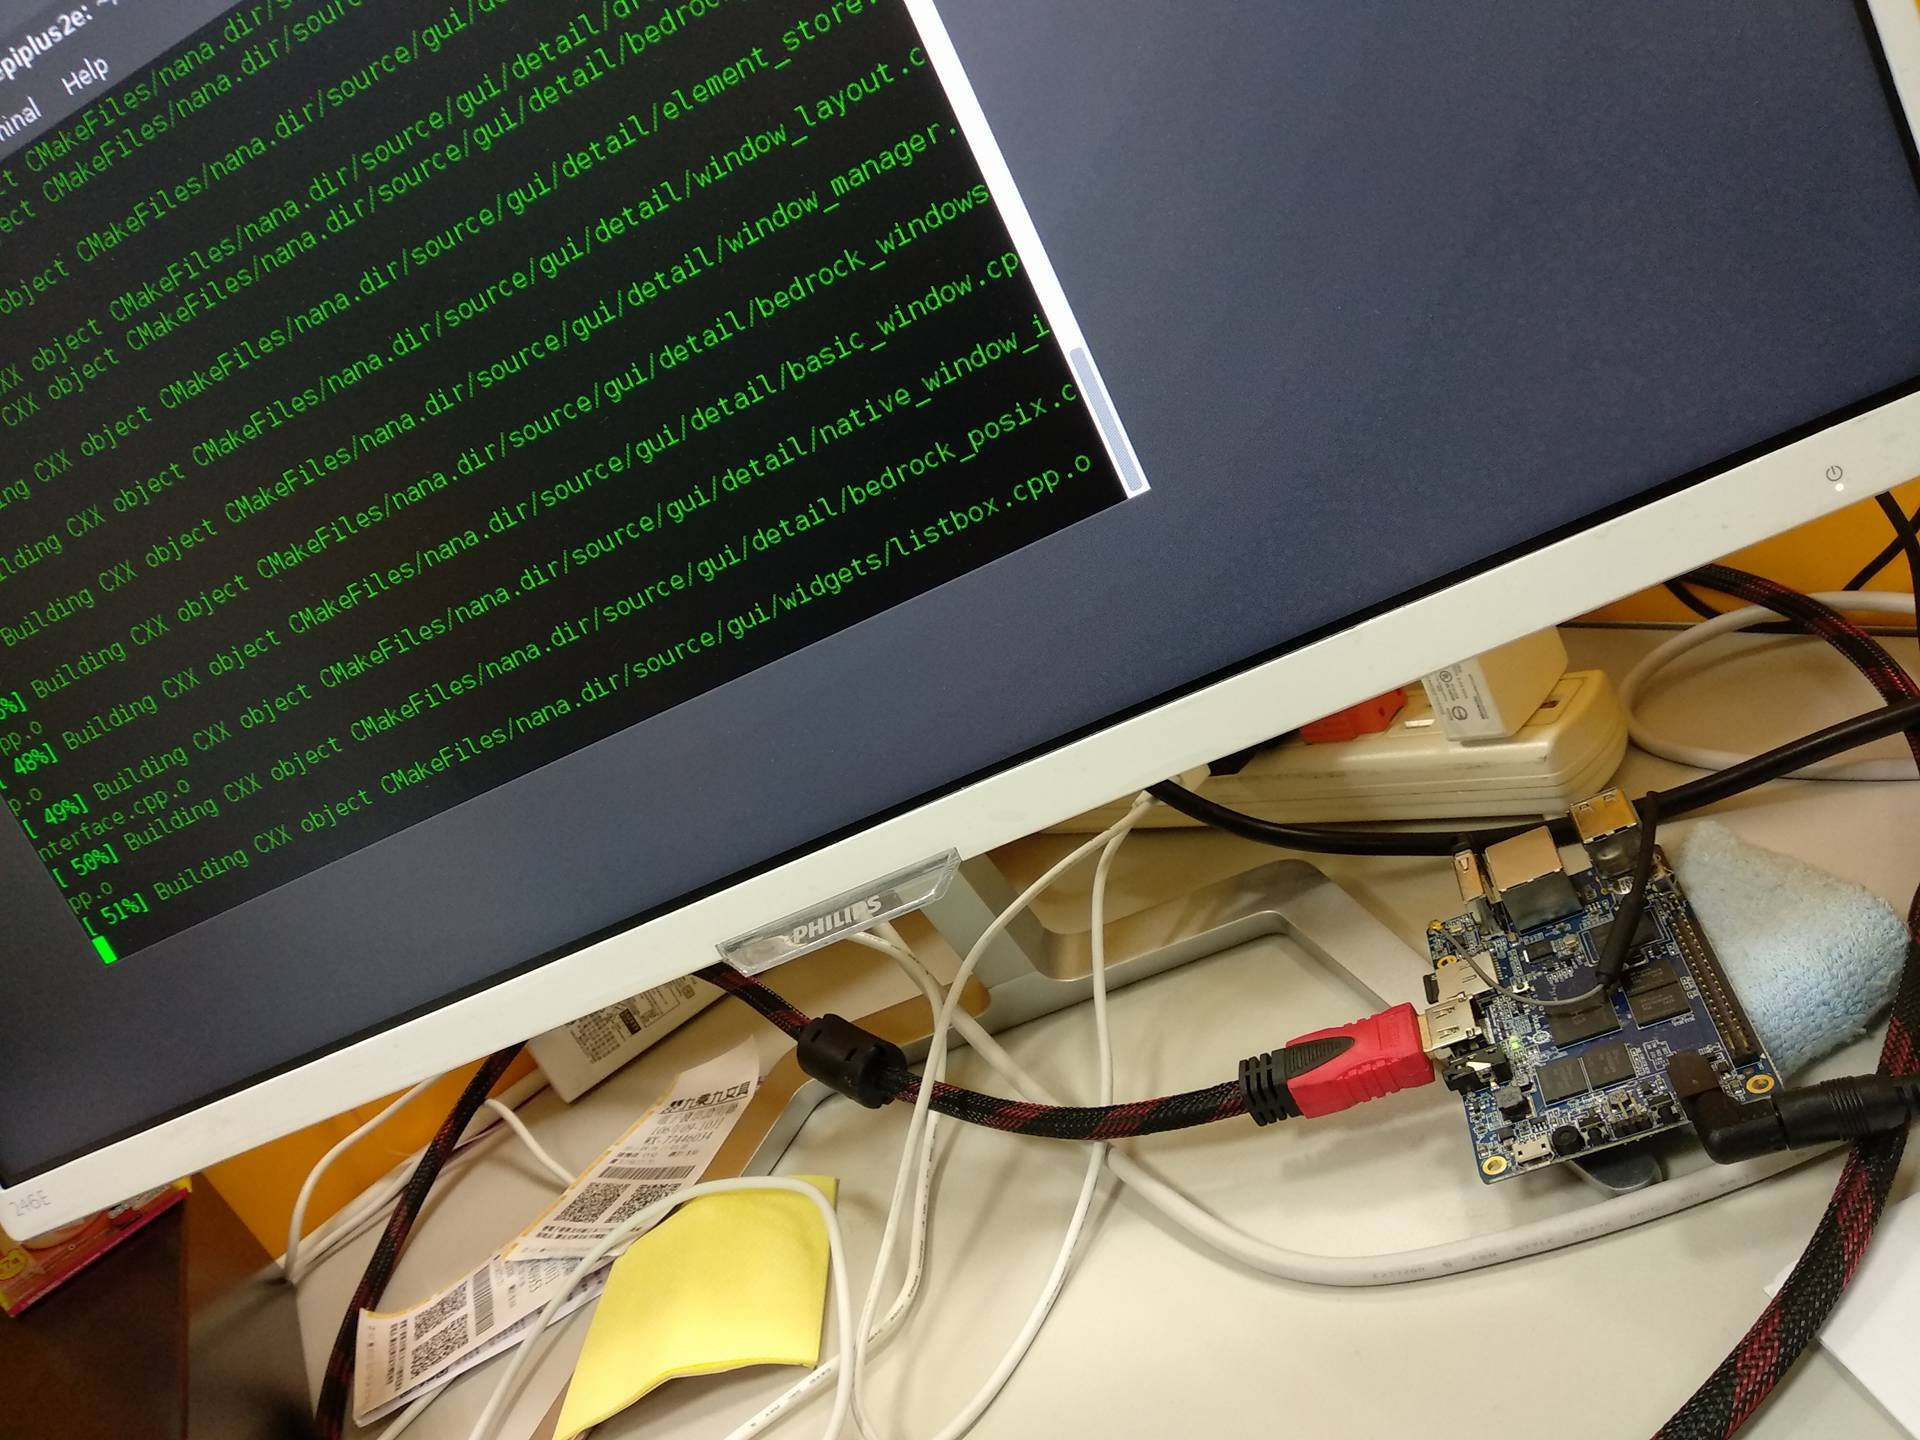
\includegraphics[width=\textwidth]{C:/Users/kevin/Desktop/workspace/docode-mdpdf/test/src/image/1.jpg}

\iffalse

\includegraphics[width=\textwidth]{1.png}
\fi

\begin{equation}
    \label{simple_equation}
    \alpha = \sqrt{ \beta }
\end{equation}

\subsection{Subsection Heading Here}
Write your subsection text here.

\section{Conclusion}
Write your conclusion here.

\section{Reference Test}
 
This document is an example of \texttt{thebibliography} environment using 
in bibliography management. Three items are cited: \textit{The \LaTeX\ Companion} 
book \cite{latexcompanion}, the Einstein journal paper \cite{einstein}, and the 
Donald Knuth's website \cite{knuthwebsite}. The \LaTeX\ related items are
\cite{latexcompanion,knuthwebsite}. 
 
\medskip
 
\begin{thebibliography}{9}
\bibitem{latexcompanion} 
Michel Goossens, Frank Mittelbach, and Alexander Samarin. 
\textit{The \LaTeX\ Companion}. 
Addison-Wesley, Reading, Massachusetts, 1993.
 
\bibitem{einstein} 
Albert Einstein. 
\textit{Zur Elektrodynamik bewegter K{\"o}rper}. (German) 
[\textit{On the electrodynamics of moving bodies}]. 
Annalen der Physik, 322(10):891–921, 1905.
 
\bibitem{knuthwebsite} 
Knuth: Computers and Typesetting,
\\\texttt{http://www-cs-faculty.stanford.edu/\~{}uno/abcde.html}
\end{thebibliography}

\end{document}